\documentclass [11pt, a4paper]{article}
\usepackage{graphicx}
\usepackage{enumerate}
\usepackage{CJK}

\title{Note of Implement Functional Languages}
\author{Hong}
\begin{document}
    \maketitle
    \tableofcontents
    \begin{flushleft}
    \newpage 
    \section{Preface}
    \begin{itemize}
        \item understand the implement of non-strict functional language
        \newline [lazy graph reduction]
        \item make functional language implementations ``come alive"
    \end{itemize}

    \subsection{Overview of the implementations}
    \begin{enumerate}
        \item source code
        \item praser  [Chapter 1]
        \item Lambda lifter [Chapter 6]
        \item core program
        \item   \begin{itemize}
                    \item Template compiler  $\rightarrow$ Template interpreter     [Chapter 2]
                    \item G-machine compiler $\rightarrow$ G-machine interpreter    [Chapter 3]
                    \item TIM ...       [Chapter 4]
                    \item Parallel G-machine ...        [Chapter 5]
                \end{itemize}
    \end{enumerate}
    
    
        \emph{interpreter.} The compiler takes a Core-language program and translates it into form suitable for execution by the machine interpreter.
        \newline
        \newline \emph{lambda lift.} It turns local function definitions into global ones, thus enabling local function definitions to be written freely and transformed out later.


    %% Chapter 1�? Core language
    \newpage
    \section{Chaptter 1: The Core Language}
    \subsection{Overview of the core language}
    \underline{\textbf{Core program}} consists of a set of \emph{supercombinator definitions}, in which \textbf{main} is a distinguished one.
    \newline Not all supercombinators have arguments. Some, such as \textbf{main}, take no arguments, which are called \emph{constant applicative forms}
    or CAFs.
    \begin{verbatim}
        main = double 21
        double x = x + x
    \end{verbatim}

    \subsubsection{Local definitions}
    Supercombinators can have local definitions:
    \begin{verbatim}
        main = quadruple 21
        quadruple x = let double_x = x + x
                      in  double_x + double_x
    \end{verbatim}

        
    \textbf{A let expression is \emph{non-recursive}}, use \textbf{letrec} for recursive definitions.
    \newline Local functions and pattern matching are not provided by Core language \textbf{let} and \textbf{letrec} executions.
    \newline
    \newline \underline{Local function} can only be defined at the top level;
    \newline \underline{Pattern matching} --- \textbf{case} expressions.
    
    \subsubsection{Structured data types}
    \emph{algebraic data types}
    \begin{verbatim}
        colour = Red | Green | Blue
        tree a = Leaf a | Branch (tree a) (tree a)
    \end{verbatim}
    Structured values are \emph{built} with constructors, and \emph{taken apart} using \emph{pattern matching}
    \newline
    \newline
    \emph{How are we to represent and manipulate structured types in small core language?}
    \begin{itemize}
        \item Use a simple, uniform representation for all constructors
        \item Transforme pattern matching into simple case expressions
    \end{itemize}

    \subsubsection{Representing constructors}
    \begin{displaymath}
        \textbf{\texttt{Pack}}\{tag, arity\}
    \end{displaymath}
    \begin{itemize}
        \item \emph{tag} is an integer to uniquely indentify the constructors
        \item \emph{arity} tells how many arguments it takes
    \end{itemize}

    \subsubsection{ \texttt{case} expressions}
    \begin{verbatim}
        -- t is a tree
        depth t = case t of
                        <1> n -> 0
                        <2> t1 t2 -> 1 + max (depth t1) (depth t2)     
    \end{verbatim}
    \texttt{case} expressions: evaluate the expression to be analysed, get the tag of the constructor it is built with and 
    evaluate the appropriate alternative.

    \subsection{Syntax of the Core Language}

    \begin{tabular}{|c|c|l|}
        \hline
        Precedence & Associativity & Operator \\
        \hline
        6 & Left & Application \\
        5 & Right & * \\
        & None & / \\
        4 & Right & + \\
        & None & - \\
        3 & None & == ~== > >= < <= \\
        2 & Right & \& \\
        1 & right & | \\
        \hline
    \end{tabular}

    \newpage
    \subsection{Structured Data Types}

    \begin{figure}[htb]
        \center {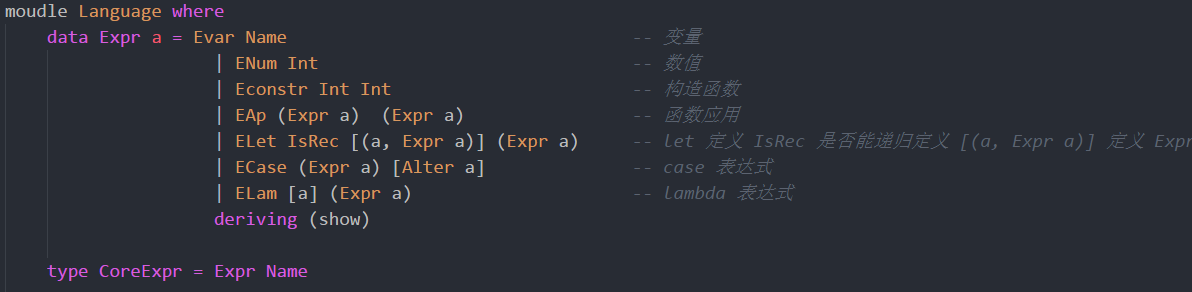
\includegraphics[width=12cm] {structured_data_types.png}}
        \caption{\label{1} structured data types}    
    \end{figure}

    \begin{verbatim}
        x + y  -> EAp (EAp (EVar) "+") (EVar "x")) (EVar "y")
    \end{verbatim}

    Definitions:
    \begin{verbatim}
    > type Name = String
    >
    > type IsRec = Bool
    > recursive, nonRecursive :: IsRec
    > recursive    = True
    > nonRecursive = False
    >
    > bindersOf :: [(a, b)] -> [a]  -- Pack(tag, arity)
    > bindersOf defns = [name | (name, rhs) <- definitions]
    > rhssOf :: [(a, b)] -> [b]
    > rhssOf defns = [rhs | (name, rhs) <- defns]
    > 
    > -- case
    > type Alter a = (Int, [a], Expr a)
    > type CoreAlt = Alter Name
    > 
    > isAtomicExpr :: Expr a -> Bool
    > isAtomicExpr (EVar v) = True
    > isAtomicExpr (ENum n) = True
    > isAtomicExpr _        = False
    > 
    > type Program a = [ScDefn a]  -- ScDefn: supercombinator definitions
    > type CoreProgram = Program Name
    > type ScDefn a = (Name, [a], Expr a)  -- [a]: argument list Expr
    > type CoreScDefn = ScDefn Name
    \end{verbatim}

    \newpage
    A small Example: 
    \begin{verbatim}
        main = double 21
        double x = x + x
    \end{verbatim}
    This program is represented by the following Haskell expression, of type \texttt{CoreProgram}
    \begin{verbatim}
[
    ("main",    [],     (EAp (EVar "double") (ENum 21))),
    ("double",  ["x"],  (EAp (EAp (EVar) "+") (EVar "x")) (EVar "x")))
]
    \end{verbatim}

    prelude definitions
    \begin{verbatim}
preludeDefs :: CoreProgram
preludeDefs = [
    ("I", ["x"], EVar "x"),
    ("K", ["x", "y"], EVar "x"),
    ("K1", ["x", "y"], EVar "y"),
    ("S", ["f", "g", "x"], EAp (EAp (EVar "f") (EVar "x"))  
                               (EAp (EVar "g") (EVar "x"))),
    ("compose", ["f", "g", "x"], EAp (EVar "f") 
                                     (EAp (EVar "g") (EVar "x"))),
    ("twice", ["f"], EAp (EAp (Evar "compose") (EVar "f")) (EVar "f"))
]
    \end{verbatim}

    \newpage
    \begin{tabular}{|lrcll|}
        \hline
        Programs & \emph{program} & $\rightarrow$ & $sc_1;...;sc_n$ & $n\geq 1$ \\
        & & & &\\
        Supercombinators & \emph{sc} & $\rightarrow$ & $var\ var_1...var_n\ =\ expr$ & $n\geq 0$ \\
        & & & &\\
        Expressions &\emph{expr} & $\rightarrow$ & \emph{expr aexpr} & Application \\
        & & $\mid$ &  $expr_1\ binop\ expr_2$ & infix binary Application \\
        & & $\mid$ &  \texttt{\textbf{let}} \emph{defns} \texttt{\textbf{in}} \emph{expr}& Local definitions \\
        & & $\mid$ &  \texttt{\textbf{letrec}} \emph{defns} \texttt{\textbf{in}} \emph{expr}& Local recursive definitions \\
        & & $\mid$ &  \texttt{\textbf{case}} \emph{expr} \texttt{\textbf{of}} \emph{alts}& Case expressions \\
        & & $\mid$ &  $\lambda var_1...var_n\ .\ expr$ & Lambda abstraction $n\geq 1$ \\
        & & $\mid$ &  \emph{aexpr} & Atomic expression \\
        & & & &\\
        &\emph{aexpr} & $\rightarrow$ & \emph{var} & Variable \\
        & & $\mid$ & \emph{num} & Number \\
        & & $\mid$ & \texttt{\textbf{Pack}}$\{num, num\}$ & Constructor \\
        & & $\mid$ & (\emph{expr}) & Parenthesised expression \\
        & & & & \\
        Definitions & \emph{defns} & $\rightarrow$ & $defn_1;...;defn_n$ & $n\geq 1$ \\
        & \emph{defn} & $\rightarrow$ & $var = expr$ & \\
        &&&&\\
        Alternatives & \emph{alts} & $\rightarrow$ & $alt_1;...;alt_n$ & $n\geq 1$ \\
        & \emph{alt} & $\rightarrow$ & $<num>\ var_1...var_n -> expr$ & \\
        
        \hline
    \end{tabular}
    \newline
    \subsection{A parser for the Core Language}
    Read a file containing the Core program in its concrete syntaxm and parse it to a value of type \texttt{CoreProgram}
    \begin{itemize}
        \item Obtain the contents of the named file as a list of characters [built-in Haskell function \texttt{read}]
        \item \emph{lexical analysis} function \texttt{lex} breaks the input into a sequence of small chunks,
        such as indentifies, numbers, symbols..., which are called \emph{tokens}
        \begin{verbatim}
> clex :: String -> [Token]
        \end{verbatim}
        \item Finally, the \emph{syntax analysis} function \texttt{syntax} consumes this sequence of tokens and 
        produces a \texttt{CoreProgram}
        \begin{verbatim}
> syntax :: [Token] -> CoreProgram     
        \end{verbatim}
    \end{itemize}

    \newpage
    \section{Chapter 2 Template instantiation}
    \begin{quotation}
        Simplest possible implementation of a functional language:
        a graph reducer base on \emph{template instantiation}
    \end{quotation}

\begin{CJK*}{UTF8}{song}
    \subsection{回顾 Template instantiation}
    \textbf{例子}
    \begin{verbatim}
        main = square (square 3)
        square x = x * x 

               @
             /   \
            @     \
           / \_____@
          *       / \
                 @   \
                / \___3
               *
          @: Application 
          ---: point
          #: point to build-in primitives
    \end{verbatim}

    \subsubsection{三步}
    \begin{enumerate}[1.]
        \item 找到下一个redex
        \item reduce 它
        \item 使用reduce的结果更新redex
    \end{enumerate}

    \emph{dump} stack of stacks, 每一个表达式的evaluate都是一个stack
    \subsubsection{Supercombinators redexs}
    Supercombinator redexs is reduced by substituting the arguments into its body; 将参数代入它的函数体内。
    \subsubsection{Constant applicative forms \textbf{(CAFs)}}

    \subsection{State transition systems}

    \newpage
    \subsection{Mark 1: A minimal template instantiation graph reducer}
    \subsubsection{transition rules}
    状态机的状态是一个四元组
    \begin{center}
        \emph{(stack, dump, heap, globals)}
    \end{center}
    简称\emph{(s,d,h,f)}
    \begin{itemize}
        \item \emph{Stack} : \emph{address}的栈, 每一个都代表一个在堆里的\emph{node} 
        \item \emph{Dump}: records the spine stack prior to the evaluation of an argument of a strict primitive;
        \item \emph{Heap}: a collection of tagged \emph{nodes}. \emph{h[a:node]} means that in the heap \emph{h}, the address a refers to the node \emph{node}
        \item \emph{Globals}: For each supercombinator (and later for each primitive), \emph{globals} gives the address of heap node representing the supercombinator(or primitive)
    \end{itemize}
    两条规则
    \begin{itemize}
        \item 展开所有的\texttt{NAp}
         \begin{verbatim}
                a:s d h[a: NAp a1 a2] f
         ==> a1:a:s d h f
        \end{verbatim}
        \item supercombinator reduction
        \begin{verbatim}
                a0:a1:...:an:s d h[a0:NSumperComb [x1,...,xn] body] f 
         ==>    ar:s d h' f
                where
                
        \end{verbatim}
        $(h', ar)\ =\ instantiate\ body\ h\ f [x_1\rightarrow a_1,...,x_n\rightarrow a_n]$
    \end{itemize}

    
\end{CJK*}
    
    \end{flushleft}
\end{document}
